 %	Skriv folgende ind som en custom Quick Build (F1)
%pdflatex -interaction=nonstopmode %.tex|bibtex %|pdflatex -interaction=nonstopmode %.tex|pdflatex -interaction=nonstopmode %.tex

\documentclass[english,twoside,openright]{report}

\usepackage[latin1,ansinew]{inputenc}
\usepackage[T1]{fontenc} 
\usepackage{babel}

\usepackage{rotating}
\usepackage[ansinew]{inputenc}
\usepackage{graphicx}
\usepackage{wrapfig}
\usepackage{float}
\usepackage{lipsum}
\usepackage{lastpage}
\usepackage{fancyhdr}
\usepackage{hyperref}    % Creates links in the PDF
\usepackage{listings}
\usepackage{algorithmic}
\usepackage{listings}
\usepackage{subfig} %til resize af billeder
\usepackage[usenames,dvipsnames]{color}
\definecolor{lightgray}{RGB}{232,232,232}
\usepackage{spverbatim} %Bruges til at indføre wrapping i kodemiljøer, ellers er den magen til {verbatim}

\lstdefinelanguage{cs}
  {morekeywords={abstract,event,new,struct,as,explicit,null,switch
		base,extern,object,this,bool,false,operator,throw,
		break,finally,out,true,byte,fixed,override,try,
		case,float,params,typeof,catch,for,private,uint,
		char,foreach,protected,ulong,checked,goto,public,unchecked,
		class,if,readonly,unsafe,const,implicit,ref,ushort,
		continue,in,return,using,decimal,int,sbyte,virtual,
		default,interface,sealed,volatile,delegate,internal,short,void,
		do,is,sizeof,while,double,lock,stackalloc,
		else,long,static,enum,namespace,string,MySQLTools,MySqlDataAdapter },
	  sensitive=false,
	  morecomment=[l]{//},
	  morecomment=[s]{/*}{*/},
	  morestring=[b]",
}

\lstdefinelanguage{nisse}
     {morekeywords={@begin,@end,@setting,fade,slide},
	  sensitive=true,
}


% CODE %
\usepackage{listings}
\usepackage{color}
\usepackage{textcomp}
\definecolor{listinggray}{gray}{0.9}
\definecolor{lbcolor}{rgb}{0.9,0.9,0.9}
\lstset{
	language=nisse,
	keywordstyle=\bfseries\ttfamily\color[rgb]{0,0,1},
	identifierstyle=\ttfamily,
	commentstyle=\color[rgb]{0.133,0.545,0.133},
	stringstyle=\ttfamily\color[rgb]{0.627,0.126,0.941},
	showstringspaces=false,
	basicstyle=\small,
	numberstyle=\footnotesize,
	numbers=left,
	stepnumber=1,
	numbersep=10pt,
	tabsize=2,
	breaklines=true,
	prebreak = \raisebox{0ex}[0ex][0ex]{\ensuremath{\hookleftarrow}},
	breakatwhitespace=false,
	aboveskip={1.5\baselineskip},
  	columns=fixed,
  	upquote=true,
 	extendedchars=true,
}


% URL %
\usepackage{url}
\makeatletter
\def\url@leostyle{\@ifundefined{selectfont}{\def\UrlFont{\sf}}{\def\UrlFont{\small\ttfamily}}}
\makeatother
\urlstyle{leo}


\setlength{\headheight}{15pt}
\pagestyle{fancy}
\renewcommand{\chaptermark}[1]{\markboth{#1}{}}
\renewcommand{\sectionmark}[1]{\markright{#1}{}}
 
 
\fancyhf{} % clear header and footer
\fancyhead[LO, RE]{\textit{\rightmark}}
\fancyhead[RO, LE]{\textit{\leftmark}}


\fancypagestyle{plain}{
\fancyhead[LE,RO,RE,LO]{}
\renewcommand{\headrulewidth}{0pt}
\fancyfoot[RO,LE]{\thepage\ of \pageref{LastPage}}}
\fancyfoot[RO,LE]{\thepage\ of \pageref{LastPage}}
% Hyppigt benyttede pakker

\usepackage{amsmath}
\usepackage{amssymb}
\usepackage{amsthm}
\usepackage{listings}
\usepackage{color}

% Farver

\definecolor{dkblue}{rgb}{0,0.1,0.5}
\definecolor{dkgreen}{rgb}{0,0.4,0}
\def\Red{\color{\ifdraft red\else black\fi}}
\def\Green{\color{\ifdraft green\else black\fi}}
\def\Blue{\color{\ifdraft blue\else black\fi}}
\def\Black{\color{black}}
\newcommand{\details}[1]{\iffull{\Blue#1}\fi}
\definecolor{linkColor}{rgb}{0,0,0.5}

% S�tninger mv.

\newtheorem{theorem}{Theorem}
\newtheorem{corollary}[theorem]{Corollary}
\newtheorem{lemma}[theorem]{Lemma}

\newtheorem{saetning}{S{\ae}tning}
\newtheorem{proposition}{Proposition}
\newtheorem{korollar}{Korollar}

\theoremstyle{definition}
\newtheorem{definition}{Definition}
\newtheorem{example}{Example}
\newtheorem{eksempel}{Eksempel}
\newtheorem{problem}[theorem]{Problem}

\newenvironment{bevis}{\begin{proof}[Bevis:]}{\end{proof}}

% Operationel semantik

\newcommand{\lag}{\langle}
\newcommand{\rag}{\rangle}
\newcommand{\setof}[2]{\ensuremath{\{ #1 \mid #2 \}}}
\newcommand{\set}[1]{\ensuremath{\{ #1 \}}}
\newcommand{\besk}[1]{\ensuremath{\lag #1 \rag}}
\newcommand{\ra}{\rightarrow}
\newcommand{\lra}{\longrightarrow}
\newcommand{\Ra}{\Rightarrow}

% M�ngdenotation

\newcommand{\pow}[1]{\mathcal{P}(#1)}
\newcommand{\Z}{\ensuremath{\mathbb{Z}}}
\newcommand{\Nat}{{\mathbb N}}
\newcommand{\Binary}{{\mathcal B}}
\newcommand{\defeq}{\stackrel{\mathrm{def}}{=}}

\newcommand{\dom}[1]{\mbox{dom}(#1)}
\newcommand{\ran}[1]{\mbox{ran}(#1)}

% Udsagnslogik

\newcommand{\logand}{\wedge}
\newcommand{\logor}{\vee}
\newcommand{\True}{\mathbf{t \! t}}

% Parenteser

\newcommand\lb {[\![}
\newcommand\rb{]\!]}
\newcommand{\sem}[1]{\lb #1 \rb}
\newcommand{\subst}[2]{\{  {}^{#1} / {}_{#1} \}}

\newenvironment{tuborg}{\left\{ \begin{array}{cc} }{\end{array} \right.}

% Flexible-length arrows (Copyright (C) 1995, Michael Rettelbach)

\makeatletter
\newdimen\lleng
\newdimen\bleng

\def\gummitrans#1{
  \setbox0=\hbox{$\stackrel{\,#1}{\mbox{}}$}
  \lleng=\wd0%
  \advance\lleng by 0.6em
  \;\raisebox{0ex}{$\stackrel{\,#1}{%
    \makebox[\lleng]{%
      \rule{0mm}{1ex}\mbox{}\leavevmode \xleaders
      \hbox {$\m@th \mkern -2.6mu \relbar \mkern -2.6mu$}\hfill\mbox{}}}$}%
  \hspace{-2.2ex}\rightarrow}

\def\Gummitrans#1{
  \setbox0=\hbox{$\stackrel{\,#1}{\mbox{}}$}
  \lleng=\wd0%
  \advance\lleng by 0.6em
  \;\raisebox{0ex}{$\stackrel{\,#1}{%
    \makebox[\lleng]{%
      \mbox{}\leavevmode \xleaders
      \hbox {$\m@th \mkern -2.6mu \Relbar \mkern -2.6mu$}\hfill\mbox{}}}$}%
  \hspace{-2.2ex}\Rightarrow}

\def\trans#1{\mathrel{\gummitrans{#1}}}
\def\Trans#1{\mathrel{\Gummitrans{#1}}}


% Bevisregler

% Med sidebetingelse

\newcommand{\condinfrule}[3]
           {\parbox{5.5cm}{$$ {\frac{#1}{#2}}{\qquad
            #3} \hfill  $$}}

% Uden sidebetingelse

\newcommand{\infrule}[2]
           {\parbox{4.5cm}{$$ \frac{#1}{#2}\hspace{.5cm}$$}}

% Regelnavn

\newcommand{\runa}[1]{\mbox{\textsc{(#1})}}

% Svar p� sp�rgsm�l

\newenvironment{svar}{\begin{quote}\noindent\textbf{Svar:}}{\end{quote}}
 %H�ttles standard-fil, anvendes den operationelle semantik
\newenvironment{boenumerate}
  {\begin{enumerate}\renewcommand\labelenumi{\textbf\theenumi}}
  {\end{enumerate}}

\begin{document}
	
	\lstset{frameround=tttt, escapeinside={\%}{\%}}
	
	
	\title{Nearly Instantaneous Slide Show Expressions}
\author{By: Group SW403F12}
\date{\emph{May 2012}}
\maketitle
\newpage
	\addtocounter{page}{1}
	\input{layout/emptypage.tex}
	\setcounter{page}{2}
	\thispagestyle{empty}
\begin{titlepage}
	\addcontentsline{toc}{chapter}{Title page}
	\setcounter{page}{3}
\begin{nopagebreak}
{\samepage 
\begin{tabular}{r}
\parbox{\textwidth}{  \raisebox{11mm}{\includegraphics[height=1.2cm]{images/aau-logo.pdf}}
\hfill \parbox{4.9cm}{\begin{tabular}{l}
{\sf\small \textbf{Department of Computer Science}}\\
{\sf\small  \textbf{Aalborg University}} \\
{\sf\small Selma Lagerl\"{o}fs Vej 300} \\
{\sf\small Telephone: +45 9940 9940} \\
{\sf\small Telefax:   +45 9940 9798} \\
{\sf\small http://cs.aau.dk}
\end{tabular}}}
\\
\end{tabular}
\vspace{-12pt}
\begin{tabular}{cc}
\parbox{7cm}{
\begin{description}

\item {\bf Title:} 

Nearly Instantaneous Slide Show Expressions
  
\item {\bf Theme:} 

Design, Definition and Implementation of Programming Language

\end{description}

\parbox{8cm}{

\begin{description}
\item {\bf Project period:}\\
   P4, Spring Term 2012\\
  \hspace{4cm}
\item {\bf Project group:}\\
  SW403F12\\
  \hspace{4cm}
\item {\bf Participants:}\\
Ali Mansour Nazim\\
Jakob Lynge Albertsen\\
Johan S�rensen \\
Jonathan Bernstorff Nielsen\\
Tommy Knudsen
  \hspace{2cm}
\item {\bf Supervisor:}\\
Benjamin Bjerre Krogh
\end{description}
}
\begin{description}
\item {\bf Circulation:} 7
\item {\bf Page count:} \pageref{LastPage}
\item {\bf Appendix count and type:} 4, Context free grammar of NISSE, ``kfG Edit'' settings, Slideshow example, Font Type
\item {\bf Finished on} May 25$^{th}$ 2012
\end{description}
\vfill } &
\parbox{7cm}{
  \vspace{.15cm}
  \hfill 
  \begin{tabular}{l}
  {\bf Synopsis:}\bigskip \\
  \fbox{
    \parbox{6.5cm}{\bigskip
     {\vfill{\small In this project, we have been developing a programming language for slideshows. Furthermore we have developed the compiler for the language, which make it possible to compile the written code to html. The main focus of the project was to make a programming language that could make it possible to make slideshows without using a pointing device, another requirement for the language was that the language should be faster to make slideshows on than already existing language such as Latex Beamer.  
     \bigskip}}
     }}
   \end{tabular}}
\end{tabular}}
\\ \\
\noindent{\footnotesize\emph{The report content is freely available, but publication (with source), only after agreement with the authors.}}
\end{nopagebreak}
\end{titlepage}
	\input{layout/signatures.tex}
	\tableofcontents	
	\addcontentsline{toc}{chapter}{Table of Contents}
	\newpage
	\chapter{Introduction}
Many people are using slideshows, in various forms, at a daily basis. There are a lot of different methods for creating a slideshow; there are programs that make it possible for the user to create slideshows relatively simple, and there are programming languages that are designed for the purpose of creating a slideshow. The software solutions for creating slideshows that will be discussed briefly are; Apple Keynote, Microsoft Office PowerPoint, \LaTeX~Beamer and NISSE (Nearly Instantaneous Slide Show Expressions). \\
A similarity that Keynote and PowerPoint have in common is that they are both pointing device based slideshow programs, which means that without using a pointing device you cannot use them properly, whereas \LaTeX~Beamer is not pointing device dependent. With \LaTeX~Beamer not being a pointing device dependent slideshow programming language makes the direct rival to the NISSE language.
A functionality that \LaTeX~Beamer lacks out on is that option for the user to use it properly at a mobile device. With �properly�� is meant that you can use it mobile, but Latex is a complex programming languages with a lot of packages, and the \LaTeX~Beamer class can use the same packages as Latex, which makes it complex to remember which packages that gives the user the exact functionality that we want. As an example of the use of packages to gain certain functionality could be that if the user wants to make a sections of his slide a certain colour, e.g. red, he has to include \usepackage{color} to make this possible. A goal with NISSE is to create a slideshow programming language where the user does not have to remember a lot of different packages to give certain functionality, or have to google how to get able to the some specific functionality. When the user has finished creating the slideshow, or if he wants to compile it, he can send it to a server that automatically compiles the slideshow for him and returns the compiled slideshow in an .HTML or .PDF-file, makes the user able to see the slideshow.\\


%\section{Server Compiler}
%A way to make the language easier to compile is to take the workload off the user's computer, and place it on a server. This creates the aspect that you can write and compile code anywhere, on any computer, or mobile device\footnote{A mobile device is defined as a laptop, tablet, smartphone, etc.}, with internet access without any additional programs.
%Having the compilation phase on a server creates the possibility to write the slideshow\footnote{The slideshow is being compiled in to one single HTML-file} on a cellphone, which can send the code to the server and receive the presentation on the device.
%With the Internet getting faster and faster\textbf{KILDE!}, more users are online, which does not limit the possibility for the users to compile their slideshows, although the compiler can be downloaded for offline use if needed.\\
\\ \\
After a walkthrough of the system, there will be a conclusion to summarize the report in general. Following this the further development section presents ideas and functionalities which could or should be implemented in the system. Included with the report is a CD containing the developed system, the source code of the developed system and the report.
	\section{Initiating Problem}
It is hard to use a pointing device\footnote{A pointing device is defined as a mouse, trackball, touchpad or pointing stick} to create slideshows while using a mobile device. To this extent, a more mobile slideshow language will be created, which will be a great way to create slideshows while ``on the go''. \\
How can a language remove the need for a pointing device when creating slideshows?
	\chapter{Problem Formulation}
%The task of making a slideshow in applications like Microsoft�s PowerPoint or Apple�s Keynote is a mouse based task. How can you make a better alternative to \LaTeX~Beamer? How can you create a programming language in which a user can make a slideshow presentation without the need for a pointing device, and not have to think about the layout of single slides, but only define the general layout. Furthermore, how can you display the presentation in a way so that it will look the same on all computers. \\
%Challenges include creating a suitable domain specific language with weight on consistency and simplicity, enabling the user to focus on the content rather than the layout.

The task of making a slideshow in applications like Microsoft�s PowerPoint or Apple�s Keynote is a mouse based task. \\
How can you make a better alternative to \LaTeX~Beamer? \\
How can you create a programming language in which a user can make a slideshow presentation without the need for a pointing device, and not have to think about the layout of single slides, but only define the general layout? \\
Furthermore, how can you display the presentation in a way so that it will look the same on all devices? \\
A challenge regarding creating a suitable domain specific language with weight on consistency and simplicity is to enable the user to focus on the content rather than the layout.
\\ \\
The following questions provide a limitation for the scope of the project:
\\ \\
Which platform should be used for presentation? \\
%Who are the users of the language? \\
Which layout decisions does the user need? \\
What are the language limitations? \\
What can be expressed in the language?
	
	% Part Analysis
	\part{Analysis}
	\chapter{Known Slideshow Applications}
In this section some of the best known applications, Microsoft PowerPoint, Apple Keynote and \LaTeX~Beamer, are compared to the solution developed during this project.
\\ \\
Microsoft PowerPoint and Apple Keynote are slideshow applications which use drag-and-drop functions, why there will be focused more on these, because this approach to create slideshows does not fulfill the requirements of being a non-pointing device based application, specified in the problem statement of this report. Because these violate the problem statement, the main focus will be on the differences between \LaTeX~Beamer and the slideshow programming language developed in this project.

\section{\LaTeX~Beamer}
An example of \LaTeX~Beamer is as follows:

\begin{lstlisting}[frame=single, caption={Beamer example}, label=lst_beamer]
%\textbf{Main\_document.tex}%
\begin{document}

\include{Slide_document.tex}

\end{document}

%\textbf{Slide\_document.tex}%
\frame {
	\frametitle{Welcome to this course}

\textit{\fontfamily{uarial}\selectfont {This course will contain information about how you \underline{underline} things, and how you do other \textit{weight stuff} on sentences.} \\
\textbf{\fontfamily{uarial}\selectfont {Like this}} \\	}
}

%\begin{figure}[H]
	\centering
		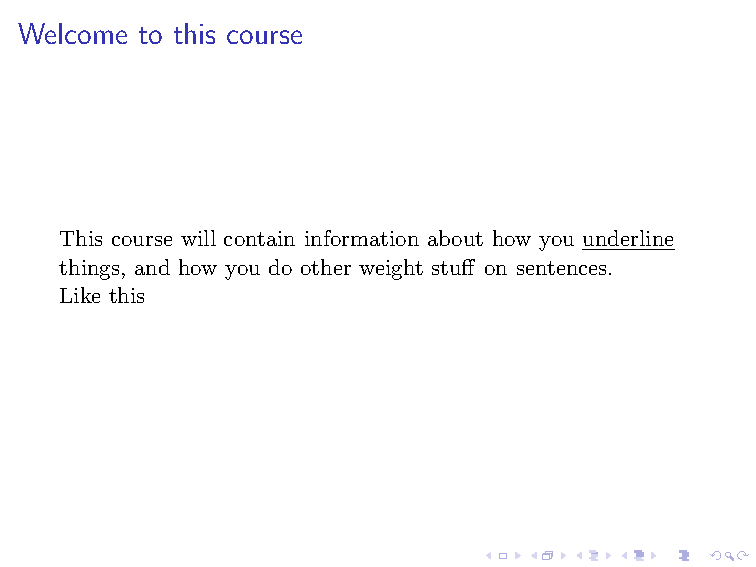
\includegraphics[width=0.8\textwidth]{text/beamer_example.pdf}
	\caption{\LaTeX~Beamer output}
	\label{fig:beamer_example}
\end{figure}%

\end{lstlisting}

The example seen in listing \ref{lst_beamer}, is the \LaTeX~Beamer-code for expressing the output. The \LaTeX~Beamer-code seen here is only to express output. To make a slideshow using \LaTeX~Beamer you have to set up a main document. In this document, all settings about; theme, colours, inputs (other files), etc., for the slideshow is set up. The editor (e.g. TexMaker), only generates a very small amount of the main document, which leaves a lot of setup for the user, if additional settings is wanted. If only a general slideshow is required, the main document will not need much work. A general slideshow is without colours, themes or the need for additional packages.\\
Compared to the \LaTeX~Beamer-code the developed language should be made more compact to make slides faster to express.
\\ \\
A test between \LaTeX~Beamer and the developed language will be made to determine which and why the one language is better than the other.

	\chapter{Language Design}
This section has been based on the book ``Concepts of Programming Languages'' \cite{CoPL}. The design of the language has been made using the language criteria in the table below. These criteria can be categorised into three primary categories; \textit{readability}, \textit{writability} and \textit{reliability}. These overall categories have a number of secondary categories, which will be used for specifying the language design. The secondary categories that affect the overall categories can be seen in table \ref{tbl:evaluation criteria}.

\begin{table}[htbp]
\centering
\begin{tabular}{|l|c|c|c|c|}
\hline
\multicolumn{1}{|c|}{\textit{Characteristics}} & \multicolumn{3}{|c|}{\textit{Criteria}} \\ \hline
 & Readability & Writability & Reliability \\ \hline
Simplicity & X & X & X \\ \hline
Orthogonality & X & X & X \\ \hline
Data types & X & X & X \\ \hline
Syntax design & X & X & X  \\ \hline
Support for abstraction & & X & X  \\ \hline
Expressivity & & X & X \\ \hline
Type checking & & & X \\ \hline
Exception handling & & & X \\ \hline
Restricted aliasing & & & X \\ \hline
\end{tabular}
\caption{Language evaluation criteria from the book ``Concepts of Programming Languages''\cite{CoPL}}
\label{tbl:evaluation criteria}
\end{table}

\noindent{\textbf{Writability}} \\
Writability is an important criterion in designing a programming language. It refers to how easy it is to write programs using the language, in the developed programming language it should be easy to write and express slideshows. A programming language is usually easier to use, if it shares some characteristics with popular languages. 
%However, a high writability ranking can also come from the language being simple to use. 
The writability has been deemed ``very important'', because our language is a slideshow programming language, and considering that a slideshow is only made once.
%otherwise there is no reason for the programmer to learn a new language to express slideshows in.
\\ \\
\textbf{Portability} \\
%Portability is also known as the ease with which programs can be implemented on another platform than the one they were originally developed for. The way to make a programming language is by standardizing the language, which can be done by focusing on readability, reliability and writability, in particular. These do not standardize the language precisely, but provide a valuable insight into the design and evaluation of the programming language in question.
Portability is also known as the ease with which programs can be implemented on another platform than the one they were originally developed for. \\
Software is portable when it is less expensive to port a program to a new platform than writing the program from scratch. The lower the cost of porting software the more portable the software is.
\\ \\
In the programming language of this project, the portability has been deemed ``very important'', because it is very important that the programming language is made in a way where it is working ``out of the box'', regardless of the operating system the programmer is using. Furthermore, the group who is to develop the programming language in question are using different operation systems, such as; Ubuntu, Mac OS X, and Windows, which makes a good foundation for checking whether the programming language is working on these three operating systems, which gives the developers a good idea of the portability of the language. Furthermore, the slides created using the system should be able to be shown on different monitor/displays.
\\ \\
\textbf{Reliability} \\
Reliability and correctness is an important criteria in designing a programming language. It refers to how reliable a programming language is. The language is reliable if it performs correctly and without errors under all conditions, in this programming language meaning that the presentation behaves exactly as the user wants it to. The ability for the language to perform correctly under all conditions, has been deemed ``important'', because the user should be able to rely on the language in a way that makes him know what it would do, using the language.
\\ \\
\noindent{\textbf{Orthogonality}} \\
Orthogonality can be seen as a consistent set of rules for combining primitive constructions. Such constructions could be to make text underlined and bold, which both are primitive constructions. \\
An example of orthogonality, from the programming language, is text formatting, which means that changes can be included not only in normal text, but also in figure text, title text, etc. \\
A high level of orthogonality makes it possible to express a lot with few primitives. \\
A low level of orthogonality results in that the user has to use many primitives to express a lot, e.g., format text in some different ways.
\\ \\
\noindent{In the programming language of this project, the orthogonality has been deemed ``important'', because it is important that there are different ways to express text formatting - making it simpler and easier to use.} \\
\\ \\
\textbf{Expressivity} \\
Is an expression covering the ease with which different operators in a programming language is designed. An example of this is using $count++$ instead of $count = count + 1$. Expressivity can
be seen as an extension to writability, in that it can make it easier to express statements in a programming language. In the developed programming language, expressivity has been deemed ``important'' because there has been a lot of focus on making the language as easy and convenient to write and express slideshows in.
\\ \\
\textbf{Readability} \\
Readability is a important criteria in designing a programming language. The definition of readability is that the language which is being designed should be easy to read and understand. When a programmer is adapting to a new language, the most difficult things to remember is usually the context of the language and the name of the data types. Creating a syntax, that in some way is similar to popular languages such as Java or C, would make the language more readable and easy to understand. \\ 
Readability of our programming language has been deemed ``less important'', because it is not as important as the writability or the reliability, though it still has to be possible to read code written in the language.
\\ \\
\textbf{Cost} \\
When talking about the cost of making a programming language, there are some different aspects to consider, these are:
\begin{enumerate}
	\item The cost of training the programmers that is going to use the language, which is a function of simplicity, orthogonality and the experience of the programmers.
	\item The cost of writing programs in the language, which is a function of writability.
	\item The cost of compiling programs in the language.
	% \item The cost of executing programs written in the language. In this part of the performance the expression ``optimization'' is introduced, which is done to in-/decrease the size and/or the execution speed of the produced code. The reason that it can in- or decrease is that; programming beginners are compiling their programs frequently, whereas more experienced programmers are, potentially, executing their programs many times after the development of a certain program.
	\item The cost of implementing the programming language.
	\item The cost of, potential, poor reliability. If, for example, a system is unreliable, it can be costly to increase its reliability.
	% \item The cost of maintaining programs written in the language, including corrections, modifications and additions to the program in question. Because maintenance is often done by other people than the original programmer, readability is of great importance, to ease the job of maintenance.
\end{enumerate}

\noindent{In the programming language of this project, the cost has been deemed ``less important'' because;}
\begin{enumerate}
	\item It is not going to be taught to other programmers than the developers, because it is a proof of concept.
	\item The only slideshows that are going to be written in the language are written by the developers themselves.
% \item As with writing programs in the language, the only programs that are going to be compiled in the language are the programs written by the developers themselves.
% \item As with writing and compiling programs in the language, the only programs that are going to be executed in the language are the programs written and compiled by the developers themselves. (if�lge vejleder)
  \item The language is not meant to be developed for bigger corporations, which is why the implementation of the language is held to a minimum.
% \item The programs in the system will not be implemented in a bigger system, as to why the implementation costs are held at a minimum.
	\item The reliability is not that big a concern for this programming language, because the slideshows written herein will not be implemented as part of a greater system, as mentioned before, but it should be seen as a proof of concept.
% \item The maintenance will be kept as close to a minimum as possible, because when slideshows have been made, using the language, these will probably not be used again, which is why it will not be necessary to maintain them.
	\item The server, from which the code is being compiled, has to have some performance, because of the possibility of multiple users creating slideshows simultaneously. The performance is not the main focus, but it is important to make sure that there will not be unnecessary waiting for the users of the programming language.
\end{enumerate}

In table \ref{tbl:evaluation criteria} is the language design criteria that has been designed for the programming language design for this project:
\begin{table}[htbp]
\centering
\begin{tabular}{|l|c|c|c|c|}
\hline
& Very important & Important & Less important & Irrelevant \\ \hline
Writability & X & & & \\ \hline
Portability & X & & & \\ \hline
Reliability & & X & & \\ \hline
Orthogonality & & X & & \\ \hline
Expressivity & & X & & \\ \hline
Readability & & & X & \\ \hline
Cost & & & X & \\ \hline
\end{tabular}
\caption{Language evaluation criteria defined for the programming language to be developed.}
\label{tbl:evaluation criteria}
\end{table}

	\section{Requirements}
\label{LanguageRequirements}
The following requirements are set for the language to consider it as a complete language:
\\ \\
\noindent{\textbf{Capabilities}} \\
\begin{itemize}
\item The language has to make it possible to make bullet points and enumerations.
\item The language has to make it possible to import pictures from the Internet.
\item The user should be able to change font- type, color, size and line height.
\item The user should be able to make a transition between each slide. 
\end{itemize}
\textbf{Error handling}\\
\begin{itemize}
\item The language should be able to tell the user which line an error has occurred. 
\end{itemize}
\textbf{Test}\\
\begin{itemize}
\item The language should be easy to write in, determined by the test:
\begin{itemize}
\item The experienced user of the language should be able to make five slides, with decent content, using standard settings, within ten minutes, where the content is prewritten.
\end{itemize}
\end{itemize}

\subsection*{Limitation}
It was estimated that it could become a source of distraction if people had too many options in the language, which would lead to a decrease in slides made per minute.

\begin{itemize}
	\item We have decided not to implement tables in our language due to the complexity of this feature.
	\item Audio is another feature, which we are not implementing in the language, because of its complexity, and because audio is not a key factor in our slideshow language.
% \item Transition of text in the slidewhoe is not necessary for a slideshow, which is why it will be left out, in the first place.
	\item Animation of text in the slideshow is not necessary for a slideshow, which is why it will be left out, in the first place.
\end{itemize}
	%\section{Types}
%Type checking for the language is redundant, because no user made variables needs to be checked, because variables cannot be created by the user. The only variables in the language are the settings, which are set to either accept a number of characters or a number of digits. Mostly any other place consists of a number of characters.
	\section{Parser Strategy}
\label{Parserstrategy}
There are two ways of parsing an abstract syntax tree, which is seen below:

\subsection*{Top Down}
Top down derives the parse tree from the left. This means that a non-terminal cannot have two derivations with the same start terminal or nonterminal, e.g. A -> BC | BD. This way the parser does not know which derivation to take, because both of them start with the same nonterminal.
This can be avoided by using a bottom up method.

\subsection*{Bottom Up}
Bottom up derives the parse tree from the right, which makes the expression: A -> BC | BD legal for a bottom up parser, because it looks at C and D first and then decides which derivation to pick.

\subsection*{Conclusion}
A top down (LL) derivation of the parser will be used in this language, because that is what the group learned first, because a useful program was introduced in a course, which could check if the parser is LL. This is beneficial in making the parser LL.
	\chapter{Lexer and Parser Generation}
In this chapter a number of lexer and parser generators will be presented, in order to determine the best generator for our project.

The lexer and parser can be made manually or generated automatically with a number of different programs. The advantage of having the lexer and parser generated by a program is that changes in the cfg can easily be implemented and checked compared to doing this manually. This will be useful when expanding the possibilities in the language, which is why a program will be used to generate the lexer and parser.

%\section{SableCC}
%A SableCC file consists of six optional sections, Package, Helpers, States, Tokens, Ignored Tokens and Productions.
%Package indicates what package the generated files should be under. Helpers are either character sets or regular expressions denoted by an identifier. Helpers can only be used in Tokens. States are used to switch between states, but are not used in this project. Tokens are defined much like Helpers. The lexer will return the longest matching token or the token listed first in Tokens if two or more tokens is matched of the same length. Ignored Tokens are tokens that are not returned by the lexer. Finally Productions are the normal production rules of the grammar, although an identifier has to be given for every alternative to a production rule, and an identifier has to be given when more then one occurrence of a production rule or token is in a given alternative.

\section{SableCC}
SableCC is a lexer and parser generator. As its input it takes an extended EBNF grammar. In order for the grammar to be accepted, the grammar has to be LALR(1), as that is the kind of parser SableCC makes. A feature of SableCC is that it can separate the generated code, from the developer's code, which makes it easy to update the compiler, as code does not have to be moved. SableCC also provides a visitor pattern to traverse the parse tree that the parser generates; this makes it easier to make the semantic analyser and the code generator.\\
A SableCC file consists of six optional sections; \texttt{package}, \texttt{helpers}, \texttt{states}, \texttt{tokens}, \texttt{ignored tokens} and \texttt{productions}.\\
\texttt{Package} indicates what package the generated files should be made using. \\
\texttt{Helpers} are either character sets or regular expressions denoted by an identifier. Helpers can only be used in \texttt{Tokens.} \\
\texttt{States} are used to switch between states, but are not used in this project. \\
\texttt{Tokens} are defined much like \texttt{Helpers}. The lexer will return the longest matching token or the token listed first in tokens if two or more tokens are matched of the same length. \\
\texttt{Ignored Tokens} are tokens that are not returned by the lexer. \\
Finally, productions are the normal production rules of the grammar, although an identifier has to be given for every alternative to a production rule, and an identifier has to be given when more than one occurrence of a production rule or token is in a given alternative.\\

\section{JavaCC}
Something Something


\section{Conclusion}
SableCC has been chosen as the lexer and parser generator, because it takes an extended EBNF grammar, which is easy to translate to from NISSE's grammar which is written in EBNF. SableCC also includes a visitor pattern, which makes it much easier to not get slowed down by not having to write the visitor pattern for all of our production rules. A SableCC specification file is also simple and easy to get started with.

	
	% Part Solution
	\part{Solution}
	\section*{Introduction}
Constructing a compiler is split into four categories; lexer, parser, semantic analyser and code generator, as shown in figure \ref{fig:Compilerconstruction}.
The user inputs some code, for the program he would like to have compiled, which is first met by the lexer. The lexer's job is to make a token for each of the characters that is provided in the code. If a character is not recognized, this stage will fail. \\

\noindent{The parser asks the lexer for a token, which is then handled by the parser. This is being repeated until there are no tokens left. The parser's main function is to check the syntax of the source code, to check whether it contains any invalid sign of formatting. The parser is doing this by creating a parse tree, which it uses to check that all tokens are given in the right order. If the parser is able to create more than one AST (Abstract Syntax tree), the code could behave differently each time it is compiled. There are also a number of ways for a parser to build an AST, which was discussed in section \ref{Parserstrategy}. If the parser fails to build an AST, this stage will fail.} \\

\noindent{The AST is then given to the semantic analyser...Something Something}

\noindent {The last phase of the compiler is the code generator. The code generator's main function is to translate the source code into the code that is chosen by the developers.}


\begin{figure}[! h]
\centering
	 \includegraphics[width=250px]{images/Compilerconstruction.png}
		 \caption{Compiler construction}
	\label{fig:Compilerconstruction}
\end{figure}




	\chapter{Syntax}
\label{SSyntax}

The requirements for the language is defined in the section ``Language design'' \ref{LanguageRequirements}. Keywords are in the language to give structure and flexibility. These have different outcomes, although some are similar. Some of the keywords are used for the structuring of slides in a slideshow, others are used for text formatting or image placement. To give a higher level of readability, keywords must have meaningful names according to their use and effect. Secondly, it has to be defined in which order these are allowed, and what they mean in that particular order.

\section{Keywords}
This is a list of reserved words in the language, where the words with the @-prefix may not be used otherwise, because the @-prefix should state that an event is about to happen.

\begin{lstlisting}[frame=single]
slide, fade, swipe, scale, rotatescale, @begin, @end, 
title, subtitle, global, text, image, url,  
#, *, 
@font_family, @font_color, @font_size, @font_weight, @u, @i, @b, 
@apply, @setting, @image, @url
\end{lstlisting}

\section{Expressions}

\subsection{@begin}
\label{@begin}
The expression \texttt{@begin} determines when a slide begins. This has a \texttt{transition} parameter separated by a pipe character, as seen in the example:
\begin{lstlisting}[frame=single]
@begin{transition|slide}
\end{lstlisting}
Where \texttt{transition} is the form of transition to the slide. 

\subsection{@end}
\label{@end}
The expression \texttt{@end} is used to determine the end of a slide, writing the line: 
\begin{lstlisting}[frame=single]
@end{}
\end{lstlisting}

\subsection{@setting}
This keyword sets a new setting for a specific type, or globally.
\begin{lstlisting}[frame=single]
@setting{FontChanges:Value | Type}
\end{lstlisting}
Where \texttt{FontChanges} is what kind of font setting that is changed. 
\texttt{FontChanges} could be font size, font family and so on, written in the language as \texttt{@font\_size} and \texttt{@font\_family} respectively. \\
\texttt{Value}, is the value that it is set to. \\
\texttt{Type} is referring to which font class it will change, e.g. title, text or the keyword. \\ %\texttt{global} in this matter means that all font classes are changed.
\texttt{Global} in this matter means that all font classes are changed.

\subsection{@apply}
The expression \texttt{apply} changes the font for some specific text.
\begin{lstlisting}[frame=single]
@apply{FontChanges:Value | Text}
\end{lstlisting}
Where \texttt{FontChanges} is what kind of font setting that is changed, and \texttt{Value}, is the value that it is set to. The difference between this and the \texttt{setting} expression is the characters after the pipe and the general meaning of the two expressions. \\
The \texttt{Text} in the expression refers to any text the user would want in this expression. \\
The \texttt{Apply} expression only changes the font for the specific text which is in the expression, whereas \texttt{@apply} only changes the font for the text inside the expression.

\subsection{@image}
%The \texttt{@image} expression imports an image from the Internet, the expression looks like this:
The \texttt{@image} expression imports an image from the internet as well as from the user's local machine, although it is discouraged to provide absolute paths for images, because this would only make the user's computer able to compile. Instead it is encouraged that the user specify the name of the image, and that he instead is placing it in the same folder as the project are in. This is only the case if there are more contributors to the slideshow.\\
When importing from the internet the URL has to be provided, whereas when importing a locally stored image the file path that specific image has to be provided, as can be seen in the example below:
\begin{lstlisting}[frame=single]
@image{@url: URL | Text }
\end{lstlisting}
%\texttt{``@url''} has to be there to indicate the start of an URL. \texttt{``URL''} indicates an URL string. \texttt{Text} refers to the text which is under the image, also called the image description.
\texttt{``@url''} is the keyword indicating that a URL will be inserted, whereas \texttt{``URL''} is the actual URL address that has been inserted. \\
The only thing that the user have to be aware of, is that the image have to be placed in the same context, or directory that the compiler if it is to function properly

\subsection{Bullet points (*)}
The \texttt{*} expression starts a list of bullet points, where the text after the star will be the text after the bullet.
A star has to be set on each line that is going to be a bullet. \\
Bullet points must never have spaces before the *, which makes the compiler think it is plain text. According to our rules, the user must not have the plain text before numerations.

\subsection{Numeration (\#)}
The \texttt{\#} expression starts a numeration list starting from one, and for each line the hash tag is used, the number is incremented. If the line after a hash tag line is not a hash tag line, the numeration list is ended and thus a new hash tag line would have its numeration starting with one. \\
Bullet points must never have spaces before the \#, which makes the compiler think it is plain text. According to our rules, the user must not have the plain text before numerations.

\subsection{Font weights}
These expressions are similar. \\
\texttt{@u} creates underlined text. \\
\texttt{@i} creates italic text. \\
\texttt{@b} creates bold text. \\
The full expression looks like this:
\begin{lstlisting}[frame=single]
@b{ Text }
\end{lstlisting}

Where \texttt{Text} is the text that is shown in the slide, with the proper change of font weight, in this case to bold. In this case a pipe is not needed because there is nothing to put there. 
It is possible to make font changes, using \texttt{@u / @i / @b}, like:

\begin{lstlisting}[frame=single]
@b{ FontChanges:Value | Text }
\end{lstlisting}

Which looks familiar to the \texttt{@apply} expression, and the functionality is basically the same, even though the text is set as any of the font weights \texttt{@u / @i / @b} to begin with. The \texttt{@u / @i / @b} makes it much faster to make a weight on a text instead of writing: @apply{ @font\_weight:bold | Text } \\
each time to make bold text.


\subsection{Hyperlink}
The expression \texttt{Hyperlink} makes it possible for the user to include URLs, either; as hyperlinks, that redirects the user to the specific URL, or image, to make it possible for the user to use an image from a specific URL.

\begin{lstlisting}[frame=single]
	@apply{@url: http://www.somelink.com/ | This URL}
\end{lstlisting}

\begin{lstlisting}[frame=single]
	@image{@url: http://media.desura.com/images/members/1/288/287053/black-1.2.jpg | Description text}
\end{lstlisting}


\subsection{Transition}
The \texttt{transition} expression is the transitions between slides. A transition can be from the actual slide to the subsequent or from the actual slide to the previous one, which can be expressed as a transition can go the left or to the right from the actual slide.

\begin{lstlisting}[frame=single]
	@begin{fade | slide}
\end{lstlisting}


\subsection{Font\_family}
The expression \texttt{font\_family} sets the font family such as Arial, Verdana, etc., from the beginning of the slideshow or at a specific slide, so that the font family can be applied locally or globally. The language supports all the font families as the CSS (Cascade Style Sheets) does.

\begin{lstlisting}[frame=single]
	@apply{@font_family: Verdana | this text is in Verdana font family}
\end{lstlisting}


\subsection{Font\_color}
The expression \texttt{font\_color} sets the font colour from the beginning of the slideshow or at a specific slide, so that the colour can be applied locally or globally. The language supports all the font colours as the CSS does.

\begin{lstlisting}[frame=single]
	@apply{@font_color: Blue| %{\color{blue}this text is in blue colour}%}
\end{lstlisting}


\subsection{Font\_size}
The expression \texttt{font\_size} sets the font size from the beginning of the slideshow or at a specific slide, so that the size can be applied locally or globally. The language supports all the font sizes as the CSS does. The font size is defined in pixels.

\begin{lstlisting}[frame=single]
	@apply{@font_size: 70 | %{\Large{this text is in size 70}}%}
\end{lstlisting}


\subsection{Font\_weight}
The expression \texttt{font\_weight} refers to the term font weight, which is the various settings that can be defined for the font, bold and italic.

\begin{lstlisting}[frame=single]
	@apply{@font_weight: italic| %\textit{this text is in italic}}
\end{lstlisting}


\subsection{Global}
The \texttt{global} expression makes it possible to apply font weights globally, from the place in the slide where it is applied or in the beginning of the slideshow. Such weights could be font colour, font family, links, etc.). Furthermore, \texttt{global} overwrites normal text, titles, subtitles, image descriptions and URL�s.
\begin{lstlisting}[frame=single]
	@setting{font_color: green | global}
\end{lstlisting}


\subsection{Title}
The expression \texttt{title} makes a title for the slide. The title can be formatted as all other text, with the different font weights, pipe, etc. The user can use the default settings for the title, regarding font family, font colour, font size, or define them himself, either at the beginning of the slideshow or at some arbitrary slide.

\begin{lstlisting}[frame=single]
	@setting{font_size: 30 | title}
\end{lstlisting}


\subsection{Subtitle}
The expression \texttt{subtitle} makes a subtitle for the slide, which means that it will be placed beneath the title, per default with a smaller font size. The subtitle can be formatted as all other text, with the different font weights, pipe, etc. The user can use the default settings for the subtitle, regarding font family, font colour, font size, or define them himself, either at the beginning of the slideshow or at some arbitrary slide.

\begin{lstlisting}[frame=single]
	@setting{font_size: 26 | subtitle}
\end{lstlisting}
%----------------------------------------------------------------------------------------------------------------------------------------&&&&&&&&&&&&&&&&&&&&&&&&&&&&&&&&&&&&&&&&&&&&&&&&&&&&&&&&&&&&&&&&&&&&&&&&&&&&&&&&&&&&&&&&&&&&&&&&&&&&&&&&&&&&&&&&&&&&&&&&&&&&&&&&&&&&&&&&&&&&&-----------------------------------------------------------------------------------------------------------------------------------------&
\section{Examples}
The following example is some of the basic elements in the language:
\begin{lstlisting}[frame=single]
Input:
@begin{fade|slide}
    Hello World
@end{slide}

%Output:Hello World%
\end{lstlisting}

Which states that a slide begins, with a transition ``fade'', and that the slide contains the text ``Hello World'' \\
The examples in the rest of this section are all written between \texttt{@begin}\{slide\} and a \texttt{@end}\{slide\} to conserve space.
\\ \\
After an @, a keyword always begins, making it easy for the compiler to recognize a keyword.
Another keyword is \texttt{setting}, in this example the setting is set for the type ``title'' to a font size of 40. \\
A setting can be initiated outside, as well as inside, a slide. The difference is that, outside a slide the setting is applied to all the upcoming slides, if the setting is inside the slide, it is only applied to that slide. If no settings are set while making the slides, default settings will be used.

\begin{lstlisting}[frame=single]
Input: @setting{@font_size:40|title}

%Output: (title font size set to 40)%
\end{lstlisting}

A way to use the title type can be as shown in the following example: \\

\begin{lstlisting}[frame=single]
Input: @title{Hello and welcome}

%Output: Hello and welcome (in the title format)%
\end{lstlisting}

Because there are no additional settings to be set on this sentence, no pipe has to occur. \\
Besides the \texttt{title} type, there is the \texttt{subtitle} type, makes a subtitle for the slide, which means that it will be placed beneath the title, per default with a smaller font size. 

\begin{lstlisting}[frame=single]
Input: @apply{@font_color:orange | funky!}

%Output:
{\color{Orange}~Funky!}
%
\end{lstlisting}

Between the left curly and the potential pipe, settings can be applied to that specific sentence, like: \\

\begin{lstlisting}[frame=single]
Input: @title{@font_size:70 |Hello and welcome}

%Output: Hello and welcome (in title format with size 70)%
\end{lstlisting}
Which sets only this line of type ``title'' to font size 70, instead of 40 which was initialized above.
This can also be applied to normal sentences like:\\

\begin{lstlisting}[frame=single]
Input: @apply{@font_size:25 | Welcome to this slide}

%Output: Welcome to this slide (with font size 25)%
\end{lstlisting}
You have to use the keyword ``apply'', to change the format of regular text. More than one format change can be applied per sentence; each format change does not necessarily need to be separated by one or more spaces. The order of format changes is irrelevant to the compiler. Here the font size is set to 25, and the text is ``Welcome to this slide''.

The weight of the text can be set in two ways, the first looks like the way we just changed the font size: \\

\begin{lstlisting}[frame=single]
Input: @apply{@font_weight:bold @font_size:25 | Welcome to bold text}

%Output: \textbf{Welcome to bold text} (with font size 25)}%
\end{lstlisting}

A quicker way to set bold text is as follows: \\

\begin{lstlisting}[frame=single]
Input: @b{Welcome to bold text}

%Output: \textbf{Welcome to bold text}%
\end{lstlisting}
Furthermore, we now want to underline a single word in that sentence: \\

\begin{lstlisting}[frame=single]
Input: @b{Welcome to @u{bold} text}

%Output: \textbf{Welcome to \underline{bold} text}%
\end{lstlisting}
Which make the whole text bold and underlines the word ``bold''.\\
Combining them, would look like this:\\

\begin{lstlisting}[frame=single]
Input: @apply{@font_weight:bold | Welcome to @u{bold} text}

%Output: \textbf{Welcome to \underline{bold} text}%
\end{lstlisting}
Which gives the same result as the last one. (e.g. ref).
\\ \\
Furthermore, it is also possible to define a specific font colour for some specific text, as can be seen as below:
\begin{lstlisting}[frame=single]
Input: @apply{@font_weight:bold @font_color:brown | Welcome to @u{bold} text}

%Output: {\color{Brown}\textbf{Welcome to \underline{bold} text}}%
\end{lstlisting}


Finally, The \texttt{global} expression makes it possible to apply font weights globally. The weights could be font colour, font family, links, etc.). Furthermore, \texttt{global} overwrites normal text, titles, subtitles, image descriptions and URL's. \\
An example of the use of \texttt{global} can be seen beneath, in this case operating with operating with  \texttt{font\_weight} and \texttt{subtitle}:

\begin{lstlisting}[frame=single]
Input:
@begin{slide}
   @setting{@font_weight:bold | global}
   @title{Hello World}
   Everything is bold!
@end{slide}

%Output:
\\ \\
\textbf{{\Large{Hello World}}
\\ \\ Everything is bold!}%
\end{lstlisting}

\subsection*{To summarize}
\texttt{@begin} To start a slide. \\
\texttt{@end} To end a slide. \\
\texttt{@b} Makes bold text. \\
\texttt{@u} Makes underlined text. \\
\texttt{@i} Makes italic text. \\
\texttt{@apply}Changes a parameter for one specific line. \\
\texttt{@setting} Changes a parameter for the slide or all upcoming slides.\\

The following is a larger example to demonstrate what is just used: \\

\begin{lstlisting}[frame=single]
Input:
@begin{fade|slide}
    @title{@b{Welcome to this course}}
    @setting{@font_family: Arial | text}
    This course will contain information about how you @u{underline} things, and how you do other    
    @i{weight stuff} on sentences.
    @apply{@font_weight:bold | Like this.}
@end{slide}


%Output:%
%\textbf{Welcome to this course} (as title)%
%This course will contain information about how you \underline{underline} things, and how you do other \textit{weight stuff} on sentences. (with font type Arial)%
%\textbf{Like this.}  (with font type Arial)%
\end{lstlisting}

Settings do not have to be set at all, if they are not set, the standard settings will be used.
%----------------------------------------------------------------------------------------------------------------------------------------&&&&&&&&&&&&&&&&&&&&&&&&&&&&&&&&&&&&&&&&&&&&&&&&&&&&&&&&&&&&&&&&&&&&&&&&&&&&&&&&&&&&&&&&&&&&&&&&&&&&&&&&&&&&&&&&&&&&&&&&&&&&&&&&&&&&&&&&&&&&&-----------------------------------------------------------------------------------------------------------------------------------------&
\section{Lists}
There are two types of lists; consisting of either bullets or numerations.
A bullet list is made by writing the following: \\

\begin{lstlisting}[frame=single]
Input:
List of things to buy
* 2 x milk
* Bread
** Light
* BKI coffee

 
%Output:\\
List of things to buy\\
\begin{itemize}
\item 2 x milk
\item Bread
\begin{itemize}
\item Light
\end{itemize}
\item BKI coffee
\end{itemize}%
\end{lstlisting}

Where a star symbolises a bullet, two bullets symbolises a bullet inside a bullet.
Numeration is made by the following: \\
Between the \texttt{\#} and the \texttt{*} the text that is related to the sign, does not necessarily need to be separated by a space, the text can also contain spaces and numbers if needed.\\

\begin{lstlisting}[frame=single]
Input:
Agenda
# Introduction
# Presentation
## Code examples
# Evaluation

%Output:\\
Agenda
\begin{enumerate}
\item Introduction
\item Presentation
\begin{enumerate}
\item Code examples
\end{enumerate}
\item Evaluation
\end{enumerate}%
\end{lstlisting}

Where a \# symbolises a number that is incrementing. Using two \# creates a sub numeration starting from one.

\section{Images}
Importing pictures from the internet and only from the internet can be done using the following code example:
% Internet
\begin{lstlisting}[frame=single]
Input: @image{@url: http://www.danwec.com/images/foto/thumbs3/aau_logo.jpg  | Aalborg University logo}

%Output:\\
(An image from the webpage \url{http://www.danwec.com/images/foto/thumbs3/aau_logo.jpg} is shown with the image description of ''Aalborg University logo'')%
\end{lstlisting}
%Internet
Importing pictures from the user's local machine can be done using the following code example:
%Local image
\begin{lstlisting}[frame=single]
Input: @image{@url: C:\Users\Benjamin\Pictures\aau_logo.jpg  | Aalborg University logo}

%Output:\\
(An image stored on the user's local machine is shown with the image description of''Aalborg University logo'')%
\end{lstlisting}
%Local image

Where the URL, or file path, to the image is placed before the pipe and after the keyword ``@url:''. The text after the pipe is the image text.
	\chapter{Lexer}
In this chapter the requirements of the lexer for NISSE will be presented, along with a listing of the tokens for NISSE.
\section{Requirements}
The requirements for the lexer are:
\begin{itemize}
		\item The lexer should be able to take any plain text file as input.
		\item The lexer should be able to recognize the input and make tokens according to the token list for NISSE.
		\item The lexer should be able to output meaningful error messages when it cannot match the input to any token.
		\item The lexer should be able to output tokens such that the parser can use them.
\end{itemize}

\newpage
\section{Token List}
In order to create the syntax in chapter \ref{SSyntax}, tokens have to be identified for later use.
\\ \\
The tokens for the language is listed in listing \ref{lst:Lexer}.

\begin{lstlisting}[frame=single, caption={Token List of NISSE in EBNF.}, label=lst:Lexer]
char            = ? [a-�A-�]+ ? ;
digit           = ? [0-9]+ ? ;
underscore      = '_' ;
hyphen          = '-' ;
dotv1           = '.' ;
commav1         = ',' ;
space           = ' ' | '	';
atsign          = '@' ;
lcurly          = '{' ;
rcurly          = '}' ;
pipe            = '|' ;
fslash          = '/' ;
bslash          = '\' ;
colon           = ':' ;
scolon          = ';' ;
blist           = '*' ;
nlist           = '#' ;
percent         = '%\%%' ;
exclamation     = '!' ;
eolv1           = \r | \n | \r\n ;
format_kwd      = '@u' | '@b' | '@i' | '@apply' | '@image' | '@title' | '@subtitle';
setting_kwd     = '@setting' ;
begin_kwd       = '@begin' ;
end_kwd         = '@end' ;
url             = '@url' ;
\end{lstlisting}
\begin{table}
\begin{center}
\begin{tabular}{|l|l|}
\hline 
Usage & Notation \\ 
\hline 
definition & = \\ 
\hline 
termination & ; \\ 
\hline 
alternation & | \\ 
\hline 
option & [ ... ] \\ 
\hline 
repetition & \{ ... \} \\ 
\hline 
grouping & ( ... ) \\ 
\hline 
terminal string & ' ... ' \\ 
\hline 
comment & (* ... *) \\ 
\hline 
special sequence & ? ... ? \\ 
\hline 
\end{tabular}
\caption{EBNF syntax}
\label{tbl:EBNFSyntax}
\end{center}
\end{table}
An example is the line \lstinline!S = a {b}+ [ {c}+ ] ( a | b ) ;! that translates to \lstinline!S = a!, followed by at least one \lstinline!b!, followed by none or at least one \lstinline!c!, followed by \lstinline!a! or \lstinline!b!. The special sequence is used for writing anything that is not directly an EBNF, defined in \ref{tbl:EBNFSyntax}. An example is \lstinline!char = ? a-�A-� ? ;! in listing \ref{lst:Lexer} where all letters from a to z is defined using both capital and non-capital. \\
\noindent{The abnormal in this token list is \lstinline!format{\_}kwd!, \lstinline!setting{\_}kwd!, \lstinline!begin{\_}kwd! and \lstinline!end{\_}kwd!, (kwd is short for ``keyword''). These keywords are explicit, because in the productions in which they occur they can only be on the left hand side of a left curly bracket. Their specific use is explained in chapter \ref{SSyntax}.}
\\ \\
The reason each expression has its own token and not a general production, is to easily see the difference between the special tokens and the normal ones, without the need to check that a given token in the syntax analyser is the right token.
\\ \\ 
\lstinline!Char! is used whenever characters needs to be used in the code. \lstinline!Char! is used both for plain text and identifiers. \\
\lstinline!Digit! is used whenever numbers need to be used in the code. \\

\subsection{NFA}
Figure \ref{fig:nfaer} is a NFA (Nondeterministic Finite Automaton) for when the user inserts an \texttt{atsign}, which can become a lot of different tokens. It will always take an input before an epsilon\footnote{The empty set.}, for instance, if an \texttt{atsign} and an \texttt{i} is written, it looks at the next tokens, before it uses the epsilon transition.

\begin{figure}[h!]
	\centering
		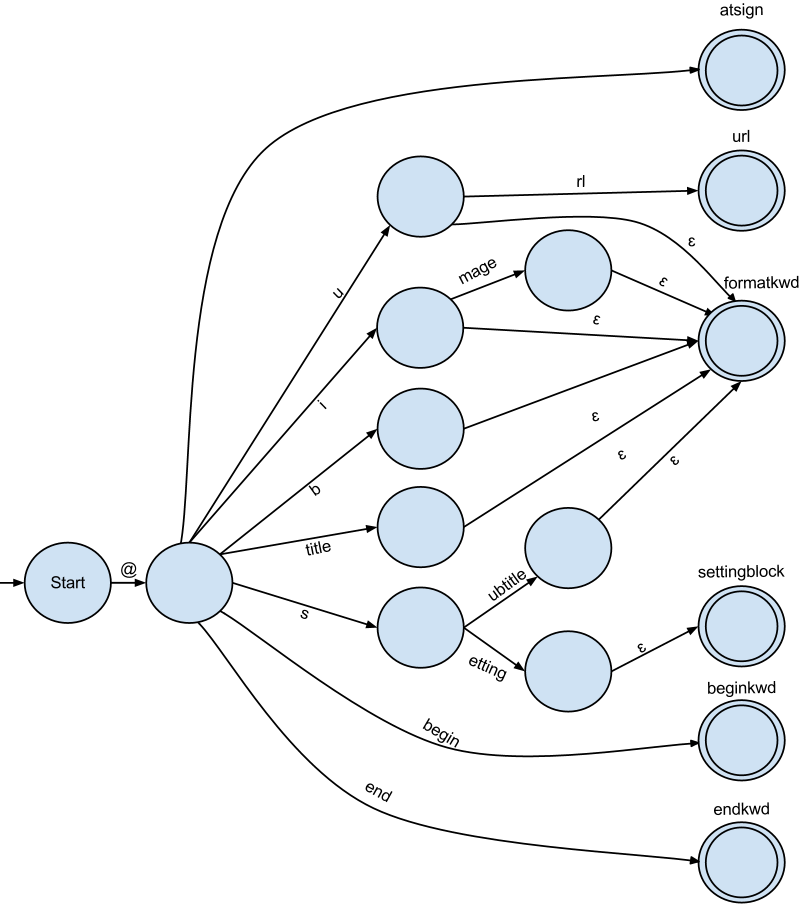
\includegraphics[width=1\textwidth]{./images/nfaer.png}
	\caption{NFA for \texttt{atsign}}
	\label{fig:nfaer}
\end{figure}

\noindent{The \texttt{atsign} can create a number of different tokens, shown in figure \ref{fig:nfaer}, these are; \texttt{formatkwd, settingblock, beginkwd, endkwd, url} and if the text does not match any of these, it is tokenized as an \texttt{atsign} and the text after the \texttt{atsign} is tokenized as a another token.}

\subsubsection*{Regular expression}
The regular expression for figure \ref{fig:nfaer} is shown in listing \ref{lst:Regularexpression}
\begin{lstlisting}[frame=single, caption=Regular expression, label=lst:Regularexpression]
%$@ ( (i (\epsilon \cup mage)) \cup (u ( \epsilon \cup rl)) \cup (b( \epsilon \cup egin) ) \cup title \cup (s(ubtitle \cup etting)) \cup end \cup \epsilon)$%
\end{lstlisting}
	\chapter{Parser}

In this chapter the requirements for NISSE will be presented, along with the CFG hereof.

\section{Requirements}
The requirements for the NISSE parser are:
\begin{itemize}
	\item The parser should be able to receive tokens from the lexer, which it then can convert into a parse tree.
	\item It should be able to report useful error messages if the user has written something illegal according to the CFG of NISSE.
	\item The CFG should be unambiguous, such that it is possible to make a parser for it. 
\end{itemize}

\newpage
\section{CFG}
\begin{lstlisting}[frame=single, caption={CFG of NISSE in EBNF.}, label={lst:ebnf}, language=NISSE]
SS              = Blocks ;
Blocks          = BeginBlock {Lines} Endblock | SettingBlock ;
Lines           = SettingBlock | Numeration | Itemlist | Plains eol ;
Numeration      = nlist (Plains eol | Numeration) ;
Itemlist        = blist (Plains eol | Itemlist) ;
BeginBlock      = beginkwd {space} BEBlock eol ;
EndBlock        = endkwd {space} BEBlock eol ;
BEBlock         = lcurly {space} char {space} [BEBlockv1] rcurly ;
BEBlockv1       = pipe {space} char {space}  ;
SettingBlock    = settingkwd lcurly ShortIdent {space} pipe {space} char {space} rcurly {space} eol ;
Plains          = (ShortBlock | CharAll) {(ShortBlock | CharAll)} ;
ShortBlock      = format_kwd lcurly {space} [ShortIdents] Plains rcurly ;
ShortIdents     = ShortIdent pipe ;
ShortIdent      = Kwd {space} colon {space} ShortIdentv1,{ShortIdentv1} {space} ;
ShortIdentv1    = char | digit | Float | colon | fslash | dot ;
Kwd             = atsign char | url ;
CharAll         = colon | digit | scolon | percent | fslash | bslash | exclamation | dot | comma | char | space | underscore | hyphen;
Float           = digit dot digit ; 
eol             = eolv1 , {eolv1} ;
dot             = dotv1 , {dotv1};
comma           = commav1,{commav1} ;
\end{lstlisting}
Listing \ref{lst:ebnf} shows the CFG for NISSE in EBNF. With the rules of table \ref{tbl:EBNFSyntax}.

NISSE's grammar is able to construct everything that is required of NISSE. \\
\begin{figure}[! h]
\centering
	 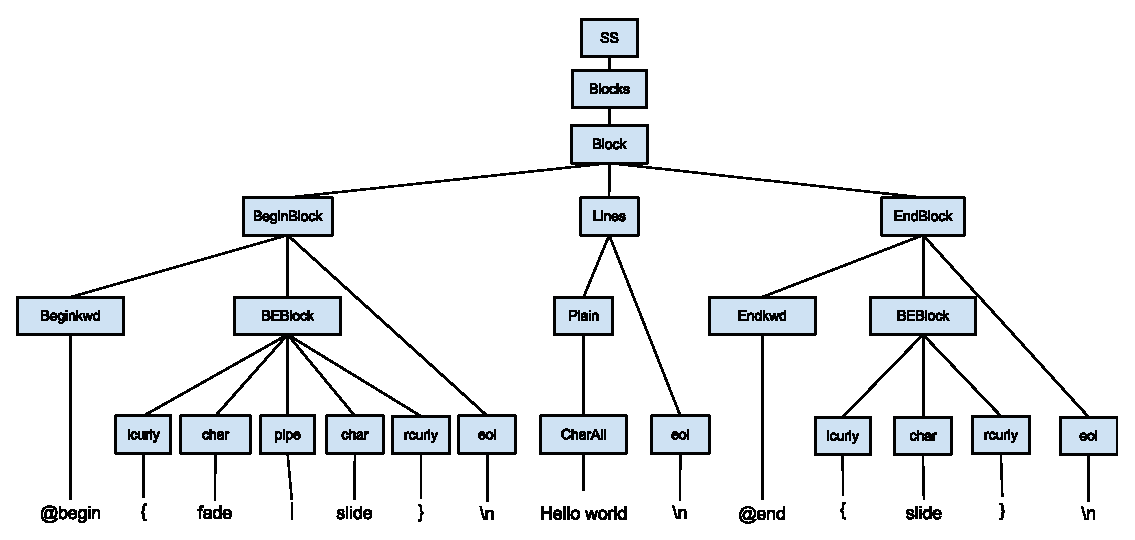
\includegraphics[width=350px]{images/ebnfexample.eps}
		 \caption{Parse tree for a simple slide.}	
	\label{fig:Parsetree}
\end{figure}
Figure \ref{fig:Parsetree} shows how the CFG would parse the AST, with the input of listing \ref{lst:BasicElemets}.
\section{Conclusion}
The CFG is concluded to be LALR according to section \ref{Parserstrategy}, the CFG is not ambiguous either, as per the definition of LALR (\cite{CaC} Chapter 6).

\noindent{The grammar for the language is LL(1) according to the tool called ``kfG Edit'', which was introduced in a lecture. Later it was tested if the grammar was LALR(1) by using SableCC to try and generate a parser, and it was proved that the grammar was LALR(1). ``kfG Edit’’ uses a special syntax that can be seen in appendix \ref{AkfG}.
	\chapter{Operational Semantics}
In this chapter some of the operational semantics of NISSE will be shown. In order to be able to read the operational semantics a few things should be known. \\
\texttt{S} denotes slides and is an environment consisting of variables (slides) pointing to a location with the \texttt{body} of the slide. \\
Also included in the environment is the keyword \texttt{next} which points to the next empty variable, and the function \texttt{new} which gets the next variable after its parameter. \\
\texttt{env} denotes an environment for settings, which also consists of variables pointing to locations containing the value of that setting. \texttt{env} does not need the \texttt{next} keyword and the \texttt{new} function because all of the settings is predefined and the only thing changed is the settings' value.
\\ \\
\noindent{$[slideshow]$}
\[ \langle S, env \rangle \ra show \]
The transition describes how the entire slideshow is made, which are with elements in \texttt{S} that has the variables in the environment.
\\ \\ 
\noindent{$[specification]$}
\[ \condinfrule{\langle slide, S \rangle \ra S' \langle setting, env \rangle \ra env'} { \langle slide~setting, S, env \rangle \ra S', env'}{} \]
This transition describes when the command slide is executed in \texttt{S}, which changes S. And when a setting is executed in the variable environment, the environment is changed.
\\ \\
\noindent{$[setting]$}
\[ \condinfrule{\langle shortident, env \rangle \ra env' \langle scope \rangle} { \langle @ setting \{ shortident | scope \}, env \rangle \ra env'}{} \]
This transition describes the inside of a setting, how the element inside a setting block changes in the variable environment in the specific scope.
\\ \\
\noindent{$[slide]$}
\[ \condinfrule{\langle block, S[L \mapsto block] [next \mapsto new L] \rangle \ra S'} { \langle block, S \rangle \ra S'}{} \]
\[ L = S(next)\]
This transition describes when a block is executed in \texttt{S}. This inserts the slide inside \texttt{S}, and moves the pointer to the next location where a slide can be inserted.
\\ \\
\noindent{$[block]$}
\[ \condinfrule{\langle setting, env \rangle \ra env' \langle plain,~S \rangle \ra S� \langle num \rangle \langle ilist \rangle} { \langle begin~setting~plain~num~ilist~end, S \rangle \ra S'}{} \]
This transition shows how commands inside a block (slide) is executed, resulting in a change in a slide.
\\ \\
\noindent{$[plain]$}
\[ \condinfrule{\langle plaintext,~S \rangle \ra S� \langle shortblock,~env \rangle \ra env'} { \langle plaintext~shortblock,~S \rangle \ra S� }{} \]
This transition illustrates how plain text and/or shortblock is evaluated, with the environment \texttt{env}.
\\ \\
\noindent{$[shortblock]$}
\[ \condinfrule{\langle formatkwd \rangle \langle shortident, env \rangle \ra env' \langle plain \rangle} { \langle formatkwd \{shortident | plain\}, env \rangle \ra env'}{} \]
This transition changes the environment according to the \texttt{formatkwd} and \texttt{shortident}, for the specific plain text.
\\ \\
\noindent{$[shortident]$}
\[ \condinfrule{\langle env [L \mapsto V] \rangle \ra env'} { \langle kwd : V, env \rangle \ra env'}{} \]
\[ L = env(kwd)\]
This transition changes the environment according to the keyword and the variable \texttt{V}.


\subsection{Derivation Tree}
An example of a derivation tree is made in figure \ref{fig:DerivationTree} of the language code in listing \ref{lst:DerivationTree}.

\begin{lstlisting}[frame=single, caption=NISSE example, label=lst:DerivationTree]
@begin{slide}
    @title{Next lecture}(1)
    @subtitle{On 15.05.2012}(2)
    This was all for now.(3)
    Have a nice day.(4) 
    The current slideshow can be found at(5) @apply{@url:http://www.somelink.com | this link }(6).
@end{slide}
\end{lstlisting}

The number at the end of almost each line i listing \ref{lst:DerivationTree} corresponds to the number in figure \ref{fig:DerivationTree}, for what it represents.

%\begin{sidewaysfigure}
%\begin{prooftree}
%\caption{Derivation Tree for listing \ref{lst:DerivationTree}
%\label{fig:DerivationTree}
%	\AxiomC{$kwd:V,~env \rightarrow env?$}
%	\AxiomC{$Plaintext,~S \rightarrow S?$}
%	\BinaryInfC{$<formatkwd\{shortident~|~Plain\},~env> \rightarrow env?$}
%	\UnaryInfC{$Shortblock,~S \rightarrow S?(1)(2)$}
%	\AxiomC{$kwd:V,~env \rightarrow env?$}
%	\AxiomC{$Plaintext,~S \rightarrow S?$}
%	\BinaryInfC{$<formatkwd\{shortident~|~Plain\},~env> \rightarrow env?$}
%	\UnaryInfC{$Shortblock,~S \rightarrow S?(6)$}
%	\BinaryInfC{$Plaintext,~S \rightarrow S?(3)(4)(5)$}
%\UnaryInfC{$begin~~~~~plain(1)~~~~~plain(2)~~~~~plain(3)~~~~~plain(4)~~~~~plain(5)~~~~~plain(6)~~~~~end$}
%	\UnaryInfC{$<slide,~S,~env> \rightarrow S?,~env?$}
%	\UnaryInfC{$<S,~env> \rightarrow show$}
%\end{prooftree}
%\end{sidewaysfigure}

The \texttt{Shortblocks} in figure \ref{fig:DerivationTree} should be seen as being on the same line as \texttt{Plaintext}.
\texttt{plain(1)} and \texttt{plain(2) } in figure \ref{fig:DerivationTree} derives to two separate shortblocks. Even though the figure only shows one shortblock, which then changes the environment, according to the shortident and formatkwd, to the \texttt{Plain}, which derives to Plaintext, and changes the content of the slide. The same goes for \texttt{plain(6)}
	\chapter{Semantic Analyser}

The semantic analyser checks for errors that the lexer and the parser do not catch. The semantic analyser for the language has the following requirements to be able to generate the expected slide.

\section{Requirements}
\begin{itemize}
	\item Check that the user defined keyword exists in the language.
	\item Check that the setting in the setting block exists.
	\item Check that it is a valid input after the colon in a setting block.
	\item Check that it is a valid scope on the right side of the pipe in a setting block.
	\item Check that the transition exists in a begin block.
	\item Check which number to put in to the enumeration.
\end{itemize}

\noindent{These requirements are put in to categories, with more explanation to specify the function of the semantic analyser.}

\section{Semantic Analysis for Text Formatting}

\subsection{Keyword Existence}
In order for the settings to work, a check to see if a specific setting actually exists in that context is needed. In order to check if the setting exists, a list of settings for a specific context is set up beforehand which it can be checked against. If the setting exists in the list, the value of the setting is checked to see if it matches a valid value of that setting. If it does not exist, an error is written to the user.


\subsection{Type Checking}
For a specific setting there is a number of valid values, two examples could be the settings \texttt{font\_size} and \texttt{font\_weight} , which sets the size or weight of a specific text, respectively. \\
In the case of \texttt{font\_size}, a valid input would be any integer. \\
In the case of \texttt{font\_weight}, a valid input would be a valid string of weight. \\
As with the keyword, existence of an error is written if the value of the setting is not valid.
The type checking for integers and integers with decimals is done by converting the value from a string to an int or float respectively.
Type checking for a specific string is done with \texttt{if} sentences, if no specific string matches any \texttt{if} sentence, an error occurs.
     
\subsection{Scope Checking}

\subsubsection*{Targeted text}
Every setting block has to be given a scope of what it is going to affect. An example could be \texttt{global}, which, for a given setting would set all types of text in the given effect level unless it is overridden at a later stage.

\subsubsection*{Effect Level}
When a setting block is inside a begin- and/or end block, the setting only affects that particular slide.\\
A setting block can also be used outside a slide, in which would make that setting apply to every slide following that specific slide, at which it is defined, unless it is overridden at a later stage. These scope settings have to be checked as to see what text the setting should apply to.

Listing \ref{LSTSemanticSetting} is a code example of when the compiler enters a setting node. The ``Visibility'' word in this section means which font type is changed; title, text, subtitle, etc.

\begin{lstlisting}[frame=single,caption=SettingBlock, label=LSTSemanticSetting, language=java]
public void inASettingblock (ASettingblock node){
	String SettingType = node.getShortident().toString().trim();
	String Visability = node.getChar().toString().trim();
	String Test = node.parent().parent().getClass().toString();
	if (Test.equals("class nisse.node.ABlockBlocks")){
		//	System.out.println("Dette er en lokal variabel");
		if (SettingType.startsWith("@ font_color")){
			String Value = SettingType.substring(15);
			Boolean CheckColor1;
			CheckColor1 = CheckColor(Value);
			if (CheckColor1 == true){
				if (Visability.equals("global")){
					SymbolTable.Scope[SymbolTable.ScopeLevel][SymbolTable.NewTextFontColor] = Value;
					SymbolTable.Scope[SymbolTable.ScopeLevel][SymbolTable.NewTitleFontColor] = Value;					
					SymbolTable.Scope[SymbolTable.ScopeLevel][SymbolTable.NewSubtitleFontColor] = Value;
					SymbolTable.Scope[SymbolTable.ScopeLevel][SymbolTable.NewImageFontColor] = Value;
					SymbolTable.Scope[SymbolTable.ScopeLevel][SymbolTable.NewUrlFontColor] = Value;
				}
				else if (Visability.equals("text")){
					SymbolTable.Scope[SymbolTable.ScopeLevel][SymbolTable.NewTitleFontColor] = Value;
				}
				else if (Visability.equals("image")){
					SymbolTable.Scope[SymbolTable.ScopeLevel][SymbolTable.NewImageFontColor] = Value;
				}
				else if (Visability.equals("title")){
					SymbolTable.Scope[SymbolTable.ScopeLevel][SymbolTable.NewTitleFontColor] = Value;
				}
				else if (Visability.equals("subtitle")){
					SymbolTable.Scope[SymbolTable.ScopeLevel][SymbolTable.NewSubtitleFontColor] = Value;
				}
				else if (Visability.equals("url")){
					SymbolTable.Scope[SymbolTable.ScopeLevel][SymbolTable.NewUrlFontColor] = Value;
				}
    	  else {
    	    System.out.println("Visability word not recognized");
    	  }
    	}
    	else {
					System.out.println("Font color:" + Value + "could not be found, try a different one, or write only with small letters");
			}
		}
		else if (SettingType.startsWith("@ font_family")){	
			String Value = SettingType.substring(16);
		�...

\end{lstlisting}


Listing \ref{LSTSemanticSetting} illustrate ``setting type''check, and changes parameters according to the ``visibility'' word, which is placed just before the right curly bracket in a setting block.\\
Line 2 fetches the setting, node \textit{Shortident}, which contains information about what setting to change and what to change it to, which is converted to a string, then the excess spaces are removed.\\
Line 3 fetches the visibility declaration, which is in the node \textit{Char}, which is also converted to a string and the excess spaces are removed.\\
Line 4 finds out which class the setting block belongs to. This is necessary to determine whether the setting block is inside or outside a slide, which is the first thing to be checked in line 5. An \textit{else} construction is made for this \textit{if} sentence which is executed when the setting should be applied on every upcoming slide.\\
Line 7 checks which keyword is going to be changed, in this case it is \textit{Font\_Color}. The parameter is then stored in a string called \textit{Value}, which takes the substring of SettingType, starting a char 15. The reason it is 15 is because a space is added after each token. So there is a space after \textit{font\_color} and a space after the colon (:) which makes the parameter start at the $15^{th}$ char.\\
Because it is a colour, it checks in the function \textit{CheckColor}, at line 9 to 11, whether the colour is allowed to be inserted. If it is not allowed, it will not change the colour, and then skip to line 38.\\
From line 12 to 33 it checks what the ``visibility'' keyword is. Depending on the word, it changes the parameter for that specific visibility.\\
Line 13 enters the document ``SymbolTable'' and the array \textit{Scope}, which inserts the parameter at the current scope level, and in the cell containing the information about text font colour.\\

\section{Semantic Analysis for Blocks}
This section focuses on blocks. A block consists of at least two lines, a \texttt{begin} line and an \texttt{end} line. Between those two lines, information can be stored. \\
The generic setup for the two lines are shown in section \ref{@begin} and \ref{@end}.

\subsection{Transition Existence}
In order for the compiler to apply a transition on a slide, the analyser has to check whether the written transition exists in the database of transitions. If the transition does not exist an error has to occur. If the transition does exist, it continues without error.

%    \subsection{Type Checking}
%The type checking in a begin- and end line consists of checking that between the two brackets is the word \texttt{slide}. In special cases, where a transition is on a slide, the word \texttt{slide} must be between the pipe and the right bracket. The word seems redundant because no other word can be in its place at this time. But for further development, where a begin- and end line can do more than just enclose a slide, this will come in handy.

\subsection{Slide type checking}
There are different types of slide layouts. For instance most slide presentations starts with a title slide, with or without a subtitle. The front page contains a title, and in some cases a subtitle, which both is in the middle of the slide. This placement is defined per default, instead of providing the user the explicit choice of this, to make it less complicated for the user. \\
The semantic analyser will check this, and creates the correct type of slide according to the text input from the user.

\begin{lstlisting}[frame=single,caption=Function: OutBlockBlocks, label=LSTOutBlockBlocks, language=java]
public void outABlockBlocks (ABlockBlocks node){
		String Transition = node.getBeginblock().toString();
		Transition = Transition.substring(9);
		String Transition1 = "none";
		if (Transition.startsWith("slide")){
		Transition1 = SymbolTable.Transition;
		}
		else if (Transition.startsWith("fade")){
			Transition1 = "fade";
		}
		else if (Transition.startsWith("swipe")){
			Transition1 = "swipe";
		}
		else if (Transition.startsWith("scale")){
			Transition1 = "scale";
		}
		else if (Transition.startsWith("rotatescale")){
			Transition1 = "rotatescale";
		}
else {
Transition1 = SymbolTable.Transition;
Error.MakeError("Transition existance" , Transition);
}
		String SlideType = "Unknown";
		Object[] Slide = node.getLines().toArray();
		int Lines = Slide.length;
		int i = 0;
		int title = 0;
		int subtitle = 0;
		int image = 0;
		while(i<Lines){
			String Slide1 = Slide[i].toString();
			if (Slide1.startsWith("@setting")  ||  Slide1.startsWith("@note")){
			}
			else if (Slide1.startsWith("@title") ) {
				title++;
			}
			else if (Slide1.startsWith("@subtitle") ) {
				subtitle++;
			}
			else if (Slide1.startsWith("@image") ) {
				image++;
			}
			else {
				SlideType = "Normal";
				SymbolTable.SlideTableAdd(SlideType, Transition1);
				indent--;
				return;
			}
			i++;
		}
		if (title > 0 && subtitle == 0 && image == 0){
			SlideType = "Title";
		}
		else if (title > 0 && subtitle > 0 && image == 0){
			SlideType = "TitleWithSubtitle";
		}
		else if (image > 0){
			SlideType = "Image";
		}		
		SymbolTable.SlideTableAdd(SlideType, Transition1);
	}
\end{lstlisting}

\subsection{Transition Existence}
	Lakslakslakslakslaks
In listing \ref{LSTOutBlockBlocks} from line 2 to 18 the function finds out if, and what, transition the slide has. In line 2 the function creates the \texttt{@begin} line to a string, which can be operated on. In line 3 it creates a substring of line 2, beginning at char 9 which is where the transition should be written, if any. Line 4 sets the transition to \texttt{none}. From line 5 it checks if the transition is \texttt{slide}, in this case there are no transition and the transition remains to be \texttt{none}. From line 10 to 18 it checks what kind of transition it is, and sets it to the found transition, if the transition is not found, the slide will have none.\\
\subsection{Slide type checking}
In listing \ref{LSTOutBlockBlocks} from line 19 to 54, we find out which type the slide it is. It starts by being \texttt{Unknown}, but it should never be that in the end. Then in line 20 it

\section{Semantic Analysis for Other Keywords}
\subsection{Image}
\texttt{Image} has to check if there exists an image on that specific url. If no image is found, accessible or in a format that is not recognized by the compiler, an error should occur.



\subsection{Enumerate}
The hash tag keyword has to keep track of the numbers, meaning that it has to increment each time a line starts with a hash tag. And when a line does not start with a hash tag, the number should start from one again. This is also applicable where hash tags are inside hash tags.

(Bliver checket i code gen)

\section{Exception Handling}




\section{Reachability and Termination Analysis}
There is no need to check for unreachable code in the language, because there are no breakers in the language e.g. return, break, exit, etc.
This also means that the language always terminates normally, because there are no keywords to stop a normal termination.



\section{SymbolTable}

in order to know the properties for each token that is written by the user, a symbol is added to the symbol table, containing the necessary information for the code generator to display the token correctly.

\begin{lstlisting}[frame=single,caption=Function: Function: SymbolTableAdd, label=LSTSemanticSymbolTableAdd]
public static void SymbolTableAdd(String Text, String Type, String FontSize, String FontFamily,String FontColor, String FontLineheight, String FontWeight, String Link){
String[] Values = {Text, Type, FontSize, FontFamily, FontColor, FontLineheight, FontWeight, Link};
SymbolTable1.put(GetCurrentSymbolNumber(), Values);
NextSymbolNumber();
}
\end{lstlisting}

Listing \ref{LSTSemanticSymbolTableAdd} shows the function called to create a symbol in the symbol table. It stores all the variables in an array which is inside a hashtable. Each hash entry has unique number in order to fetch the entry. before the function ends the number is incremented by 1, which is the next unique hashkey.


\section{SlideTable}
An additional table is created to keep track of the overall properties in a slide, meaning the transition between the slides, and which type of slide it is, eg. a title page or a normal page.
The slide type is determined in listing \ref{LSTOutBlockBlocks}. In line 56 in listing \ref{LSTOutBlockBlocks}, it calls the function SlideTableAdd, which is shown in listing \ref{LSTSlideTableAdd}. Where the transition at the beginning is set to \texttt{none}, but can be modified in the function \texttt{outABlockBlocks} in listing \ref{LSTOutBlockBlocks}. The slide table looks more or like the symbol table, only with fewer elements in the array.

\begin{lstlisting}[frame=single,caption=Function: Function: SlideTableAdd, label=LSTSlideTableAdd]
static String Transition = "none";

public static void SlideTableAdd(String Type, String Transition){
			String[] Values = {Type, Transition};
			SymbolTableForSlide.put(GetSlideNumber(), Values);
			NextSlide();
		}  
\end{lstlisting}

	\chapter{Code Generator}

The code generator takes the decorated AST from the semantic analysis and with it, it generates the output code. In the case of NISSE, the output from the code generator is a mixture of HTML (Hypertext Markup Language), CSS and JavaScript. The code generator has the following requirements in order for it to generate a correct slideshow.

\section{Requirements}
\begin{itemize}
  \item Print out the header of the HTML-files, along with the necessary libraries needed for the slideshow to function.
  \item Retrieve and print out the global settings from the symbol table into the header of the HTML-file.
  \item Retrieve information about slide type and slide transition from the slide table about all of the slides.
  \item Print out all of the plain text, numeration and item lists with the right settings, according to the symbol table.
  \item Keep track of when to open and close tags, such that correct HTML is output, while keeping the file as small as possible.
  \item End the HTML-file and output the generated code to the output file.
\end{itemize}
Each of these requirements will be described further in the following subsections.

\section{Header File and Libraries}
The common header file of all generated slides is kept in a data file called \texttt{prefix} inside the compiler. The header file consists of; HTML metatags, the common CSS of all slides, the JavaScript libraries and the start of the body of the HTML-file. \\

\noindent{The HTML metatags are there so that the slideshows work on mobile devices (e.g. Apple Iphone/Ipad or Android phones/tablets), because without them the slideshows would not scale correctly for the mobile device screens. The metatags also disables user zoom so that the user can use swipes to change slide without the need to worry about placement or size of the slide.} \\

\noindent{The common CSS of all slides is mainly how the page itself is setup, how a slide looks and the background colour.} \\

\noindent{A few JavaScript libraries are used to make the slideshows work, these libraries are; jQuery and a plugin for jQuery called Touchswipe. \\
jQuery is mainly used to facilitate all of the transitions of the slides, e.g., it makes it easy to animate CSS attributes. \\
jQuery is also used to change CSS attributes. The plugin Touchswipe is used to make it possible to use swipe motions on mobile devices to change slide, which would otherwise not be possible.} \\

\noindent{A custom library is also included which uses jQuery and Touchswipe to implement the different transitions. A key hook is set up so that when the user presses a button, the code checks to see if the user pressed any of the buttons to change the slide. A similar \texttt{swipe hook} is set up using Touchswipe, to catch user swipes and check what direction the swipe was in. These hooks then calls a common function called \texttt{go\_to\_slide} which sends the user to the requested slide. The \texttt{go\_to\_slide} function checks the \texttt{data-transition} tag of the requested slide to check which transition to run. The function then calls the appropriate function which will then change to the requested slide with the given transition. The last thing included in the custom library is so that when desktop or laptop users resize their windows, the slide and text size is automatically scaled down so that the slide still fits the whole window.} \\

\section{Transitions}
Currently the compiler supports four different types of transitions between slides. These are; fade, swipe, scale and rotatescale. All of the animations required for the transitions are done through jQuery. NISSE supports the use of different transitions on slides in the same slideshow. The way this is done is that the first slide in the slideshow is placed in the centre of the screen, while the rest of the slides are moved 100 \% down to a slide stack and is hidden. The reason the rest of the slides are moved 100 \% down is that there is a limitation in HTML so that if elements are hidden above other elements, the user is not able to click at hyperlinks. Each transition moves the slides into place in order for the animation to work.\\
The fade transition starts by moving the slide it is switching to, to the middle of the screen (while it is still hidden). Using jQuery the CSS option opacity is then animated to 0 for the current slide. After that animation has finished the next slides' opacity is then animated to 1, making it visible. Finally the previous slide is moved back to the slide stack. \\
The swipe transition starts by moving the slide it is switching to, to either the left or right of the screen (depending on whether the user is moving forward or backwards in the slides) and moves the slide up to the centre of the screen. The current slide is then animated either to the left or right, while the next slide is animated into the centre of the screen. While this is going on, the current slides' opacity is animated to 0, while the next slides' is animated to 1. Finally, the previous slide is moved back to the slide stack. \\
The scale transition starts by moving the slide it is switching to, to the middle of the screen. The scale transition makes use of the CSS option transform, which is implemented in major browsers using their own \texttt{tag}. In order to support all of the major browsers, all four versions of the transform option is animated. The four versions are; \\ \\
\texttt{-webkit-transform} for all browsers built upon webkit (e.g. Chrome or Safari), \\
\texttt{-moz-transform} for all of the Mozilla browsers, \\
\texttt{-o-transform} for the Opera browser, and \\
\texttt{-ms-transform} for all of the Microsoft browsers. \\ \\
The option of transform used is the \texttt{scale()} option. Because jQuery can only animate numeric CSS options, a workaround is used in order to animate the scale option. A CSS option that is not used in this context (in this case \texttt{border-spacing}) is animated in the range wanted, and every time the animate function steps another function is called which modifies the transform option with the value that the animate function has reached. At the same time, the next slide is faded in. Finally the previous slide is then moved back to the slide stack. \\
The rotatescale transition works similarly to the scale transition, but while animating the scale option it also animates the rotate option. Like all other transitions, the previous slide is moved back to the slide stack.

\section{Global settings}
The NISSE specification allows for the use of settings in a \texttt{global} scope. These settings need to be output in the header of the HTML file. The code generator retrieves the global settings from the symbol table, converts them to CSS code and outputs them into the header of the HTML file.

\section{End of the header}
All of the previous code was all placed inside the \texttt{header} of the HTML file. The code generator now starts the \texttt{body} of the file and outputs the \texttt{wrapper} of the slides.

\section{Starting slides}
Slides in the HTML-file are wrapped in a \texttt{div} that has the class \texttt{slide\_wrapper}. The div also has to have some tags set in order for the slideshow to work. The first one is the id of the div, each slide has to have a unique id starting with slide0 and incrementing the number for every slide, this is used when the slideshow moves to a slide. \\
The second tag is the \texttt{data-transition} tag, which specifies what transition should be used when moving \texttt{away} from that slide. \\
The last tag that has to be set is the style of the div. The first slide of the slideshow is placed in the middle of the screen and is visible, specified by the CSS \texttt{top:0\%; opacity:1;}. The rest of the slides is placed 100 \% below the screen and is hidden, specified by the CSS \texttt{top:100 \%; opacity:0;}. \\
The slides is then also wrapped in a div with the class equal to the type of slide, i.e. titleslide, imageslide.

\section{Printing out plain text}
Because most of the work figuring out what the style of plain text should be is done in the semantic analyser, the code generator part of printing out plain text is relatively simple. All of the style for text can be retrieved from the symbol table. The only challenge is figuring out when to open and close tags in the HTML-file. Because text has to be surrounded with tags the code generator has to check when to close tags when new text is met, instead of when moving ``out'' of the text. Using this method the code generator is also able to reduce the amount of code outputted by only starting a new \texttt{span} when the style of text changes. Titles and subtitles are also special in that style can change while still in the same title, which means that \texttt{span} has to be used inside titles in order for style to change inside it.

\section{Ending the HTML-file}
After all of the slides have been generated, the last thing the code generator does is output some last HTML-tags in order to close out the HTML-file.

	
	%\input{text/parser/Parser}
	
	\part{Appendix}
	\appendix{}
	\chapter{kfG}
\label{AkfG}
Listing \ref{lst:akfG} is the settings used in the program ``kfG Edit'', to be able to write ASTSableCC grammar for examples of the defined language.
This is an older iteration of the cfg, which means it does not fit into the latest one.
\begin{lstlisting}[frame=single, caption=kfG grammar for the language, label=lst:akfG]
SS           -> Blocks 
Blocks       -> Block Blocks | EPSILON 
Block        -> BeginBlock Lines EndBlock | SettingBlock
Lines        -> Line Lines | SettingBlock Lines | EPSILON 
Line         -> List | Plains eol
List         -> Numeration | Itemlist 
Numeration   -> nlist Numv1 
Numv1        -> Plains eol | Numeration 
Itemlist     -> blist Itemv1 
Itemv1       -> Plains eol | Itemlist 
BeginBlock   -> beginkwd BEBlock eol
EndBlock     -> endkwd BEBlock Eols
BEBlock      -> lcurly BEBlockv1 pipe Ident Space  rcurly
BEBlockv1    -> Ident Space | EPSILON
SettingBlock -> settingkwd lcurly Kwd colon Settingv1 Space pipe String rcurly eol
Settingv1    -> Ident| Number
Plains       -> Plain Plains | EPSILON
Plain        -> ShortBlock | CharSpace | Number
ShortBlock   -> Kwd lcurly ShortIdents pipe Plains rcurly
ShortIdents  -> ShortIdent | EPSILON 
ShortIdent   -> Kwd colon Settingv1 Space ShortIdents
String       -> CharSpace Stringv1
Stringv1     -> String  | EPSILON
CharSpace    -> char | pace
Ident        -> char Identv1
Identv1      -> Ident | EPSILON
Number       -> digit Numberv1
Numberv1     -> Number | EPSILON
Kwd          -> atsign Ident
Space        -> pace Space | EPSILON
CharAll      -> colon | char | digit | nlist | blist | scolon | percent | fslash | bslash
Eols         -> eol Eolv1
Eolv1        -> Eols | EPSILON


pace       -> ' ' 
settingkwd -> '@setting'
beginkwd   -> '@begin'
endkwd     -> '@end' 
atsign     -> @
lcurly     -> { 
rcurly     -> } 
seperator  -> <> 
pipe       -> '|' 
fslash     -> /
bslash     -> \
colon      -> : 
scolon     -> ; 
blist      -> * 
nlist      -> # 
percent    -> %\%%
eol        -> \n | \r | \r\n 
char       -> a|b|...|z|A|B|...|Z| _ |.|,
digit      -> 0|1|...|9
\end{lstlisting}

\chapter{CFG(SableCC)}
\label{SableCC}
Listing \ref{lst:aSableCC} is the settings used in the program ``SableCC'', to generate the lexer and parser for the language.
\begin{lstlisting}[frame=single, caption=SableCC grammer for the language, label=lst:aSableCC]
Package nisse;

Helpers
       charv1    = ['a' .. 'z'] | ['A' .. 'Z'] | '�' | '�' | '�' | '�' | '�' | '�';
       digitv1   = ['0' .. '9'] ;
       dot         = '.' ;
       comma       = ',' ;
       eolv1     = 13 10 | 13 | 10;

Tokens
       format_kwd  = '@u' | '@b' | '@i' | '@apply' | '@image' | '@title' | '@subtitle' | '@note' ;
       url         = '@url' ;
       space       =  ' ' | 9 ;
       settingkwd  = '@setting' ;
       beginkwd    = '@begin' ;
       endkwd      = '@end' ;
       atsign      = '@' ;
       lcurly      = '{' ;
       rcurly      = '}' ;
       pipe        = '|' ;
       fslash      = '/' ;
       bslash      = '\' ;
       colon       = ':' ;
       scolon      = ';' ;
       blist       = '*' ;
       nlist       = '#' ;
       percent     = '%\%%' ;
       exclamation = '!' ;
       underscore  = '_' ;
       hyphen      = '-' ;
       eol         = eolv1+;
       char        = charv1+ ;
       digit       = digitv1+ ;
       float       = digitv1+ dot digitv1+ ;
       dot         = dot+;
       comma       = comma+ ;

Productions 
       nisse         = blocks* ;
       blocks        = {block} beginblock lines* endblock 
                     | {setting} space* settingblock ;
       lines         = {setting} settingblock 
                     | {numeration} numeration
                     | {itemlist} itemlist 
                     | {plaintext} plains eol ;
       numeration    = nlist numerationv1 ;
       numerationv1  = {plaintext} plains eol 
                     | {numeration} numeration;
       itemlist      = blist itemlistv1 ;
       itemlistv1    = {plaintext} plains eol  
                     | {itemlist} itemlist;
       beginblock    = beginkwd space* beblock [second]:space* eol ;
       endblock      = endkwd space* beblock [second]:space* eol ;
       beblock       = lcurly [first]:space* char [second]:space* beblockv1? rcurly ;
       beblockv1     = pipe [first]:space* char [second]:space*;
       settingblock  = settingkwd lcurly shortident pipe [second]:space* char [third]:space* rcurly space* eol;
       plains        = plainsv1+;
       plainsv1      = {shortblock} shortblock 
                     | {charall} charall;
       shortblock    = format_kwd space* lcurly shortidents? plains rcurly ;
       shortidents   = shortident+ pipe ;
       shortident    = kwd space* colon [first]:space* shortidentv1+ [second]:space*;
       shortidentv1  = {char} char 
                     | {digit} digit
                     | {float} float
                     | {colon} colon
                     | {fslash} fslash
                     | {dot} dot
                     | {underscore} underscore
                     | {hyphen} hyphen;
       kwd           = {at} atsign kwdv1+
                     | {url} url ;
       kwdv1         = {char} char
                     | {underscore} underscore;
       charall       = {colon} colon
                     | {digit} digit
                     | {float} float
                     | {semicolon} scolon
                     | {percent} percent
                     | {forwardslash} fslash
                     | {backslash} bslash
                     | {exclamation} exclamation
                     | {dot} dot 
                     | {comma} comma
                     | {char} char
                     | {space} space 
                     | {underscore} underscore
                     | {hyphen} hyphen;
\end{lstlisting}

	\bibliographystyle{plain}
	\bibliography{kilder}
	\addcontentsline{toc}{chapter}{Bibliography}
	\newpage
	\appendix
	\input{layout/emptypage.tex}

\end{document}
